\documentclass{beamer}

\usepackage[francais]{babel}
\usepackage[utf8]{inputenc}
\usepackage[T1]{fontenc}
\usepackage{graphicx}
\usepackage{graphics}
\usepackage{color}
\usepackage{textcomp}
\usepackage{pifont}
\usepackage[normalem]{ulem}
\usepackage{times}
\usepackage{hyperref}
\usepackage{verbatim}
\usepackage{amsmath}
\usepackage{amsthm}
\usepackage{amsfonts}
\usepackage[mathscr]{euscript}
\usepackage{pgfpages}
\usepackage{listings}
\usepackage{subfigure}
\usepackage{algorithm}
\usepackage[noend]{algorithmic}
\usepackage{pdftricks}
\usepackage{mathrsfs}
\usepackage{array}
\usepackage{fancybox}
% \usepackage{columns}
\usepackage{multirow}
\usepackage{url}
\usepackage{tikz}
\usepackage{colortbl}
%\usepackage{cite} %DO NOT FUCKING USE CITE ON BEAMER !!! LOST 30 GODDAM' MINUTES ON THIS SHIT !!!
\usepackage{mathabx}
\usepackage{amssymb}
\usepackage{eurosym}
\usepackage{wasysym} % ch0

\let\texteuro\euro

\hypersetup{colorlinks,%
            citecolor=black,%
            filecolor=black,%
            linkcolor=black,%
            urlcolor=blue}

%\addtolength{\parskip}{10pt}

\usetikzlibrary{calc}

\mode<presentation>
\setbeamertemplate{footline}[frame number]
\setbeamercovered{transparent}
\usetheme[navigation]{ESI}

%lst
\definecolor{comment-green}{RGB}{0,166,80}
\lstset{language=C++,
  keywordstyle=\lst@ifdisplaystyle\bf\fi\color{blue!60},
  commentstyle=\color{comment-green},
  stringstyle=\color{red},
  basicstyle=\lst@ifdisplaystyle\tiny\else\tt\fi,
  morekeywords={
    constexpr,concept,decltype,nullptr,nullptr_t,noexcept,final,override},
  frame=single,
  xleftmargin=0.5cm,
  numbers=left,
  tabsize=2}

%title
\subtitle{Langage \texttt{C} / \cpp}
\author{R. Absil}
\date{\today}

%styles
\theoremstyle{definition}
\newtheorem{thm}{Théorème}
\newtheorem{conj}[thm]{Conjecture}
\newtheorem{deff}[thm]{Définition}
\newtheorem{prop}[thm]{Propriété}
\newtheorem{lem}[thm]{Lemme}
\newtheorem*{lem*}{Lemme}
\newtheorem{cor}[thm]{Corollaire}
%\newtheorem{example}{Exemple}
\newtheorem{remark}{Remarque}
\newtheorem{exo}{Exercice}

%typeset
\newcommand{\ie}{{\emph{i.e., }}}
\newcommand{\eg}{{\emph{e.g., }}}
\newcommand{\etal}{{\emph{et al.}}}
\newcommand{\rrceil}{\unichar{"2308}}
\newcommand{\sloand}[2]{\footnote{N. J. A. Sloane - OEIS Foundation - \texttt{www.oeis.org}, Sequence #1 - #2.}}

%math
\newcommand{\IN}{{\mathbb N}}
\newcommand{\IQ}{{\mathbb Q}}
\newcommand{\IR}{{\mathbb R}}
\newcommand{\IZ}{{\mathbb Z}}
\newcommand{\IP}{{\mathbb P}}
\newcommand{\IC}{{\mathbb C}}
\newcommand{\bigo}{{\mathcal{O}}}
\renewcommand{\mod}{\bmod}
\newcommand{\ssi}{\Leftrightarrow}
\newcommand{\then}{\Rightarrow}
\newcommand{\fle}[1]{\stackrel{#1}{\longrightarrow}}
\newcommand{\suchthat}{~\big|~}
\newcommand{\floor}[1]{\left\lfloor #1 \right\rfloor}
\newcommand{\ceil}[1]{\left\lceil #1 \right\rceil}
\DeclareMathOperator*{\argmin}{argmin}
\DeclareMathOperator*{\argmax}{argmax}

%tikz
\tikzstyle{_vertex}=[fill=white, circle,minimum size=12pt,inner sep=1pt]
\tikzstyle{_blackv}=[fill=black, circle,minimum size=8pt,inner sep=1pt]
\tikzstyle{_dot}=[fill=black, circle, minimum size = 1mm, inner sep=0pt]
\tikzstyle{_bigvertex}=[fill=white, circle,minimum size=21pt,inner sep=1pt]
\tikzstyle{_arc}=[->, >=stealth]
\tikzstyle{_boldarc}=[->, >=stealth, line width=2pt]

\newcommand{\cpp}{\texttt{C++}}
\newcommand{\java}{\texttt{Java}}


\title{Ch. 12 - Héritage et polymorphisme}

\begin{document}
\begin{frame}
  \titlepage
\end{frame}

\begin{frame}
  \frametitle{Table des matières}
  \footnotesize \tableofcontents[pausesections,pausesubsections]
\end{frame}


\section{Introduction}

\begin{frame}
\frametitle{Overview}
\begin{itemize}[<+->]
\item Un des fondements de la POO
\item Permet de « transférer » la signature d'une classe dans une autre
\item En jargon \cpp, on parle souvent de \emph{classe dérivée} et de \emph{classe de base} plutôt que de sous-classe et de super-classe.
\end{itemize}
\begin{exampleblock}<+->{Dérivation en \cpp}
	\begin{itemize}[<+->]
	\item Via « \texttt{:} » après le nom de la classe
	\item \lstinline|class B : A \{ ... \};|	
	\item Appels super-constructeurs via la liste d'initialisation
	\end{itemize}
\end{exampleblock}
\begin{itemize}[<+->]
\item Plusieurs « types » de dérivation possible
	\begin{itemize}
	\item Définit la visibilité des membres de la classe de base
	\end{itemize}
\end{itemize}
\end{frame}

\begin{frame}
\frametitle{Différences entre \java\ et \cpp}
\begin{itemize}[<+->]
\item En \cpp, il n'y a pas d'interfaces
	\begin{itemize}
	\item Classes abstraites sans attributs
	\end{itemize}
\item En \cpp, l'héritage multiple est autorisé
	\begin{itemize}
	\item Attention aux ambiguïtés
	\end{itemize}
\item Le polymorphisme n'est pas « activé » par défaut
	\begin{itemize}
	\item Il faut dire explicitement quelles fonctions membres sont polymorphiques
	\item Il faut que l'objet soit alloué dynamiquement, ou une référence
	\end{itemize}
\item Conversion implicite de type « tronquage » d'une classe dérivée vers une classe de base
	\begin{itemize}
	\item Pour les objets automatiques uniquement
	\end{itemize}
\end{itemize}
\end{frame}

\begin{frame}[containsverbatim]
\frametitle{Exemple}
\begin{itemize}
\item Fichier \texttt{pointcol.cpp}
\end{itemize}
\begin{lstlisting}
class point
{
	int x, y;
	
	public:
		point(int x = 0, int y = 0) : x(x), y(y) {}		
		void setLocation(int x, int y) { this -> x = x; this -> y = y; }
		friend ostream& operator <<(ostream& out, const point& p)
		{ out << "( " << p.x << " , " << p.y << " )"; }	
};

class pointcol : public point
{
	short r, g, b;
	
	public:
		pointcol(int x, int y, short r, short g, short b) : point(x,y), r(r), g(g), b(b) {}
};

int main()
{
	pointcol p(1,2,80,0,0); cout << p << endl;
	p.setLocation(3,4); cout << p << endl;	
}
\end{lstlisting}
\end{frame}

\section{Principes}

\begin{frame}
\frametitle{Différents types de dérivation}
\begin{itemize}[<+->]
\item Trois types de dérivation
	\begin{enumerate}
	\item Dérivation publique : \lstinline|class B : public A \{ ... \};|
		\begin{itemize}
		\item Les membres publics de \texttt{A} sont accessibles comme membres publics dans \texttt{B}
		\item Les membres protégés de \texttt{A} sont accessibles comme membres protégés dans \texttt{B}
		\end{itemize}
	\item Dérivation privée : \lstinline|class B : private A \{ ... \};|
		\begin{itemize}
		\item Les membres publics et protégés de \texttt{A} sont accessibles comme membres privés dans \texttt{B}
		\end{itemize}
	\item Dérivation protégée : \lstinline|class B : protected A \{ ... \};|
		\begin{itemize}
		\item Les membres publics et protégés de \texttt{A} sont accessibles comme membres protégés dans \texttt{B}
		\end{itemize}
	\end{enumerate}
\item En l'absence de spécificateur d'accès, la dérivation est
	\begin{itemize}
	\item publique pour les \lstinline|struct|
	\item privée pour les \lstinline|class|
	\end{itemize}
\end{itemize}
\end{frame}

\begin{frame}
\frametitle{Spécificateurs d'accès et amitié}
\begin{itemize}[<+->]
\item Le mot-clé \lstinline|protected| permet au membre spécifié d’être accédé uniquement par le concepteur d’une sous-classe
\item Résolution de portée via \texttt{::}
\item Une classe dérivée n’a jamais accès aux membres privés de sa classe de base
	\begin{itemize}
	\item Sauf si une relation d'amitié est déclarée
	\end{itemize}
\item Possibilité de définir un membre dans une classe à l'aide de \lstinline|using|
	\begin{itemize}
	\item Permet de changer la visibilité d'un membre dans une sous-classe
	\item Éviter
	\end{itemize}
\item Possibilité de définir une classe dérivée comme amie d'une classe de base
	\begin{itemize}
	\item Permet à une sous-classe d'accéder aux membres privés de sa classe de base
	\end{itemize}
\end{itemize}
\end{frame}

\begin{frame}[containsverbatim]
\frametitle{Exemple 1}
\begin{itemize}
\item Fichier \texttt{specifier.cpp}
\end{itemize}
\begin{lstlisting}
class A
{	
	public:
		void printA() { cout << "A"; }
};

class B : public A
{
	public:
		void printB() 
		{ 
			printA(); //ok : printA is a public member of this
			cout << "B";
		}
};

int main()
{
	A a; a.printA(); cout << endl;
	B b; b.printB(); b.printA(); cout << endl; //ok : printA is a public member of B
}
\end{lstlisting}
\end{frame}

\begin{frame}[containsverbatim]
\frametitle{Exemple 1}
\begin{itemize}
\item Fichier \texttt{specifier.cpp}
\end{itemize}
\begin{lstlisting}
class C : private A
{
	public:
		void printC() 
		{ 
			printA(); //ok : printA is a private member of this
			cout << "C";
		}
};

class D : public C
{
	public:
		void printD()
		{
			//printA(); //ko : printA is a private member of superclass
			cout << "D";
		}	
};

int main()
{
	C c; c.printC(); cout << endl; //c.printA(); //ko : printA is a private member of C
	D d; d.printD(); cout << endl; //d.printA(); //ko : printA is a private member of D
}
\end{lstlisting}
\end{frame}

\begin{frame}[containsverbatim]
\frametitle{Exemple 1}
\begin{itemize}
\item Fichier \texttt{specifier.cpp}
\end{itemize}
\begin{lstlisting}
class E : protected A
{
	public:
		void printE() 
		{ 
			printA(); //ok : printA is a protected member of this
			cout << "E"; 
		}
};

class F : public E
{
	public:
		void printF()
		{
			printA(); //ok : printA is a protected member of superclass
			cout << "F";
		}	
};

int main()
{
	E e; e.printE(); cout << endl; //e.printA(); //ko : printA is a protected member of E
	F f; f.printF(); cout << endl; //f.printA(); //ko : printA is a protected member of F
}
\end{lstlisting}
\end{frame}

\begin{frame}[containsverbatim]
\frametitle{Exemple 2}
\begin{itemize}
\item Fichier \texttt{using.cpp}
\end{itemize}
\begin{lstlisting}
class A 
{ 
	protected : 
		int i; 
	public:
		A(int i = 0) : i(i) {}
};

class B : public A 
{
	public:		
		using A::i; 
		using A::A;
};

int main()
{
	B b(4); cout << b.i << endl;
	b.i = 3; cout << b.i << endl;
}
\end{lstlisting}
\end{frame}

\begin{frame}
\frametitle{Amitié et héritage : rappel}
\begin{alertblock}<+->{Règles}
\begin{itemize}[<+->]
\item Les relations d'amitié ne sont pas transitives
	\begin{itemize}
	\item L'ami d'un ami n'est pas votre ami
	\end{itemize}
\item L'amitié n'est pas propagée par héritage
	\begin{itemize}
	\item Les enfants de votre ami ne sont pas vos amis	
	\item Vos enfants ne sont pas les amis de votre ami
	\end{itemize}
\item À partir de \cpp11, les amis ont accès aux classes internes privées
\end{itemize}
\end{alertblock}
\begin{itemize}[<+->]
\item Souvent, un choix de design est effectué pour soit
	\begin{enumerate}
	\item rendre une classe \texttt{B} entière amie d'une autre classe \texttt{A}
	\item faire d'une classe \texttt{B} une classe interne d'une autre classe \texttt{A}
	\end{enumerate}
\item Cf. Ch. 7
\end{itemize}
\end{frame}

\begin{frame}[containsverbatim]
\frametitle{Exemple}
\begin{itemize}
\item Fichier \texttt{friend.cpp}
\end{itemize}
\begin{lstlisting}
class A
{
	int _i;
	
	public:
		A() : _i(2) {}
		int i() const { return _i; }

		friend class M; //class M is a friend of A
};

class B : public A
{
	int _j;
	
	public:
		B() : _j(3) {}
		int j() const { return _j; }
};
\end{lstlisting}
\end{frame}

\begin{frame}[containsverbatim]
\frametitle{Exemple}
\begin{itemize}
\item Fichier \texttt{friend.cpp}
\end{itemize}
\begin{lstlisting}
//M is a friend of A and not a friend of its children
class M
{
	int _k;

	public:
		M(A a) : _k(a._i * 2) {}
		//M(B b) : _k(b._j * 3) {}

		int k() const { return _k; }
};

//children of M are neither friends of A or B
class N : public M
{
	int _l;

	public:
		N(A a) : M(a)/*, _l(a._i * 4)*/ {}
		N(B b) : M(b)/*, _l(b._j * 5)*/ {}

		int l() const { return _l; }
};
\end{lstlisting}
\end{frame}

\section{Redéfinition et surdéfinition}

\begin{frame}
\frametitle{Redéfinition des membres d'une classe dérivée}
\begin{itemize}[<+->]
\item Pour redéfinir un membre d'une classe dérivée, il suffit de le déclarer avec le même prototype que celui de la classe de base.	
	\begin{itemize}
	\item Le membre de la classe de base est alors « caché ».
	\end{itemize}
\item Un appel au membre sur la classe dérivée appelle le membre redéfini.
\end{itemize}
\begin{exampleblock}<+->{Exemple}
	\begin{itemize}
	\item \lstinline|struct A \{ void print() \{ ... \} \};|
	\item \lstinline|struct B : A \{ void print() \{ ... \} \};|
	\item \lstinline|B b; b.print(); //calls B::print|
	\end{itemize}
\end{exampleblock}
\begin{itemize}[<+->]
\item \lstinline|final| empêche la redéfinition d'un membre dans une classe dérivée, ou la dérivation d'une classe
\end{itemize}
\end{frame}

%\item Possibilité d'empêcher la dérivation d'une classe via \texttt{final} (\cpp11).
%\item Permet également d'empêcher la redéfinition d'une fonction dans une classe dérivée.

\begin{frame}
\frametitle{Accès aux membres et transtypage}
\begin{itemize}[<+->]
\item Accès aux membres via \texttt{b.print()} (dérivé) et \texttt{b.A::print()} (classe de base).
\item Aucune correspondance polymorphique n'est effectuée par défaut !
	\begin{itemize}
	\item On ne peut pas mettre un \texttt{B} automatique dans un \texttt{A} automatique.
		\begin{itemize}
		\item Si on le fait = « tronquage des membres » (taille)
		\end{itemize}
	\item Si on met un \texttt{B} dynamique (pointeur) dans un \texttt{A} dynamique, on ne peut appeler que les membres de \texttt{A}.
		\begin{itemize}
		\item Même comportement avec les références
		\end{itemize}
	\item Plus de détails dans la section « Polymorphisme »
	\end{itemize}
\end{itemize}
\end{frame}

\begin{frame}[containsverbatim]
\frametitle{Exemple}
\begin{itemize}[<+->]
\item Fichier \texttt{no-poly.cpp}
\end{itemize}
\begin{lstlisting}
class point
{
	protected:
		int x, y;
	
	public:
		point(int a = 0, int b = 0) : x(a), y(b) {}

		void print()
		{ cout << "( " << x << " , " << y << " )" << endl; }
};

class pointcol : public point
{
	short r, g, b;	
	public:
		pointcol(int x = 0, int y = 0, int r = 255, int g = 255, int b = 255) 
			: point(x,y), r(r), g(g), b(g) {}

		void print()
		{ 
			cout << "( " << x << " , " << y << " ) - color : " 
				<< r << " , " << g << " , " << b << endl; 
		}
};
\end{lstlisting}
\end{frame}

\begin{frame}[containsverbatim]
\frametitle{Exemple}
\begin{itemize}
\item Fichier \texttt{no-poly.cpp}
\end{itemize}
\begin{lstlisting}
int main()
{
	point p(3,5);	
	pointcol pc (8,6,255,128,128);	

	p.print();
	pc.print();

	p = pc; //truncated
	p.print(); //no polymorphism

	point * ptp = &p;
	pointcol * ptpc = &pc;
	ptp = ptpc; //no polymorphism
	ptp -> print();	
	
	point & rp = p;
	pointcol & rpc = pc;
	rp = rpc;
	rp.print(); //no polymotphism
}
\end{lstlisting}
\end{frame}

\begin{frame}
\frametitle{Redéfinition et surdéfinition}
\begin{exampleblock}<+->{Redéfinition (overiding)}
	\begin{itemize}[<+->]
	\item Réécriture du prototype d'un membre d'une classe de base au sein d'une classe dérivée.
	\end{itemize}
\end{exampleblock}
\begin{exampleblock}<+->{Surdéfinition (overloading)}
	\begin{itemize}[<+->]
	\item Réécriture du prototype d'un membre, souvent au sein d'une même classe.	
		\begin{itemize}
		\item Seul autre cas : réécriture du prototype d'un membre \texttt{final} d'une classe de base dans une classe dérivée.
		\end{itemize}
	\end{itemize}
\end{exampleblock}
\begin{itemize}[<+->]
\item Le compilateur effectue une résolution des liens et décide quelle fonction appeler
\end{itemize}
\end{frame}

\begin{frame}
\frametitle{Résolution des liens lors d'héritage}
\begin{itemize}[<+->]
\item Les liens sont résolus dans l'ordre suivant :
	\begin{enumerate}
	\item Appel direct (correspondance exacte).
%		\begin{itemize}
%		\item Correspondance exacte, appel explicite potentiel.
%		\end{itemize}
	\item Conversion de paramètre et appel direct avec le converti.
		\begin{itemize}
		\item Uniquement si une conversion implicite est possible.
		\end{itemize}
	\item Appel de base (correspondance exacte).
%		\begin{itemize}
%		\item Appel du membre de la classe de base.
%		\end{itemize}
	\item Conversion de paramètre et appel de base avec le converti.
		\begin{itemize}
		\item Uniquement si une conversion implicite est possible.
		\end{itemize}
	\end{enumerate}
\end{itemize}
\begin{alertblock}<+->{Remarque importante}
	\begin{itemize}[<+->]
	\item Si on appelle une fonction membre dans une classe dérivée surdéfinissant une fonction dans la classe de base, le compilateur appelle \emph{toujours} la fonction de la classe dérivée
		\begin{itemize}
		\item Si ce n'est pas possible, erreur de compilation
		\end{itemize}
	\end{itemize}
\end{alertblock}
\begin{itemize}[<+->]
\item Comportement très différent en \java
\end{itemize}
\end{frame}

\begin{frame}[containsverbatim]
\frametitle{Exemple 1}
\begin{itemize}
\item Fichier \texttt{linkres-1.cpp}
\end{itemize}
\begin{lstlisting}
class A
{
	public:
		void f(int n)
		{
			cout << "int " << n << endl;
		}

		void f(char n)
		{
			cout << "char " << n << endl;
		}
};

class B : public A
{
	public:
		void f(float x)
		{
			cout << "float " << x << endl;
		}
};
\end{lstlisting}
\end{frame}

\begin{frame}[containsverbatim]
\frametitle{Exemple 1}
\begin{itemize}
\item Fichier \texttt{linkres-1.cpp}
\end{itemize}
\begin{lstlisting}
int main()
{
	int n = 1;
	char c = 'a';
	A a;
	B b;
	
	a.f(n);
	a.f(c);
	b.f(n);
	b.f(c);
}
\end{lstlisting}
\end{frame}

\begin{frame}[containsverbatim]
\frametitle{Exemple 2}
\begin{itemize}
\item Fichier \texttt{linkres-2.cpp}
\end{itemize}
\begin{lstlisting}
class A
{
	public:
		void f(int n)
		{
			cout << "A::int " << n << endl;
		}

		void f(char n)
		{
			cout << "char " << n << endl;
		}
};

class B : public A
{
	public:
		void f(int n)
		{
			cout << "B::int " << n << endl;
		}
};
\end{lstlisting}
\end{frame}

\begin{frame}[containsverbatim]
\frametitle{Exemple 2}
\begin{itemize}
\item Fichier \texttt{linkres-2.cpp}
\end{itemize}
\begin{lstlisting}
int main()
{
	int n = 1;
	char c = 'a';
	B b;
	
	b.f(n);
	b.f(c);
}
\end{lstlisting}
\end{frame}

\begin{frame}[containsverbatim]
\frametitle{Exemple 3}
\begin{itemize}
\item Fichier \texttt{linkres-3.cpp}
\end{itemize}
\begin{lstlisting}
class A
{
	public:
		void f(int n)
		{
			cout << "A::int " << n << endl;
		}

		void f(char n)
		{
			cout << "char " << n << endl;
		}
};

class B : public A
{
	
};
\end{lstlisting}
\end{frame}

\begin{frame}[containsverbatim]
\frametitle{Exemple 3}
\begin{itemize}
\item Fichier \texttt{linkres-3.cpp}
\end{itemize}
\begin{lstlisting}
int main()
{
	int n = 1;
	char c = 'a';
	B b;
	
	b.f(n);
	b.f(c);
}
\end{lstlisting}
\end{frame}

\begin{frame}[containsverbatim]
\frametitle{Exemple 4}
\begin{itemize}
\item Fichier \texttt{linkres-4.cpp}
\end{itemize}
\begin{lstlisting}
class A
{
	public:
		void f(int n)
		{
			cout << "A::int " << n << endl;
		}

		void f(char n)
		{
			cout << "char " << n << endl;
		}
};

class B : public A
{
	public:
		void f(int n, int m)
		{
			cout << "int,int " << n << " " << m << endl;
		}
};
\end{lstlisting}
\end{frame}

\begin{frame}[containsverbatim]
\frametitle{Exemple 4}
\begin{itemize}
\item Fichier \texttt{linkres-4.cpp}
\end{itemize}
\begin{lstlisting}
int main()
{
	int n = 1;
	char c = 'a';
	B b;
	
	b.f(n);
	b.f(c);
}
\end{lstlisting}
\end{frame}

\section{Construction, destruction, affectation}

\begin{frame}
\frametitle{Ordre d'appel}
\begin{itemize}[<+->]
\item Soient \texttt{A} une classe de base et \texttt{B} une classe dérivée.
\item Quand on crée/copie/déplace un objet \texttt{B}, on appelle, dans cet ordre :
	\begin{enumerate}
	\item le constructeur de \texttt{A},
	\item le constructeur de \texttt{B}.
	\end{enumerate}
\item Quand on détruit un objet \texttt{B}, on appelle, dans cet ordre :
	\begin{itemize}
	\item le destructeur de \texttt{B},
	\item le destructeur de \texttt{A}.	
	\end{itemize}
\item Pour les constructeurs et destructeurs par défaut, les appels sont faits implicitement.
\item Pour les constructeurs avec paramètres, il faut les appeler via la liste d'initialisation.
\end{itemize}
\end{frame}

\begin{frame}[containsverbatim]
\frametitle{Exemple}
\begin{itemize}
\item Fichier \texttt{constr-destr.cpp}
\end{itemize}
\begin{lstlisting}
struct A
{
	A() { cout << "+A()"<< endl; }
	A(int a) { cout << "+A(int)" << endl; }
	~A() { cout << "-A()" << endl;}		
};

struct B : A
{
	B() { cout << "+B()" << endl; }
	B(int a, int b) : A(a) { cout << "+B(int,int)" << endl; }			
	~B() { cout << "-B()" << endl; }
};

int main()
{
	A a; A aa(2);
	B b; B bb(2,2);
}
\end{lstlisting}
\end{frame}

\begin{frame}
\frametitle{Constructeur de recopie / déplacement}
\begin{exampleblock}<+->{Rappel}
\begin{itemize}[<+->]
\item Le constructeur de recopie est appelé quand
	\begin{enumerate}
	\item on initialise un objet par un autre de même type (explicite),
	\item on passe un objet par valeur à une fonction (implicite).
	\end{enumerate}
\end{itemize}
\end{exampleblock}
\begin{itemize}[<+->]
\item Les règles d'appel liées au constructeur sont aussi valides pour le constructeur de recopie.
\item Il faut néanmoins tenir compte de certaines subtilités selon que le constructeur de recopie a été redéfini ou non.
\item Même principe avec le constructeur de déplacement
\item Dans les exemples suivants, \texttt{B} dérive publiquement de \texttt{A}.
\end{itemize}
\end{frame}

\begin{frame}
\frametitle{Absence de constructeur de recopie dans la classe dérivée}
\begin{itemize}[<+->]
\item Appel du constructeur de recopie par défaut de \texttt{B}.
	\begin{itemize}
	\item Rappel : la recopie se fait membre à membre.
	\item Les données pointées par les attributs dynamiques ne sont pas recopiées.
	\end{itemize}
\item La « partie » de \texttt{B} qui « appartient » à \texttt{A} est traitée comme un membre de type \texttt{A}.
\end{itemize}
\begin{exampleblock}<+->{Règle}
\begin{itemize}[<+->]
\item Le constructeur de recopie de la classe de base est appelé implicitement.
\end{itemize}
\end{exampleblock}
\begin{itemize}[<+->]
\item S'il existe, il est appelé.
\item Sinon : constructeur de recopie par défaut. 
\end{itemize}
\end{frame}

\begin{frame}[containsverbatim]
\frametitle{Exemple}
\begin{itemize}
\item Fichier \texttt{no-recop.cpp}
\end{itemize}
\begin{lstlisting}
class point
{
	protected:
		int x, y;	
	public:
		point(int a = 0, int b = 0) : x(a), y(b) {}
		point(const point& p) : x(p.x), y(p.y) { cout << "+r point" << endl; }
		friend ostream& operator << (ostream& out, const point& p)
		{ 
			out << "( " << p.x << " , " << p.y << " )"; 
		}
};

class pointcol : public point
{
	short r, g, b;	
	public:
		pointcol(int x = 0, int y = 0, int r = 0, int g = 0, int b = 0) 
			: point(x,y), r(r), g(g), b(b) {}
		friend ostream& operator << (ostream& out, const pointcol& p)
		{ 
			out << "( " << p.x << " , " << p.y << " ) - color " 
			    << p.r << " " << p.g << " " << p.b; 
		}
};
\end{lstlisting}
\end{frame}

\begin{frame}[containsverbatim]
\frametitle{Exemple}
\begin{itemize}
\item Fichier \texttt{no-recop.cpp}
\end{itemize}
\begin{lstlisting}
void f(pointcol p) 
{ 
	cout << "f" << endl; 
}

int main()
{
	pointcol a(1,2,3);
	f(a);
}
\end{lstlisting}
\end{frame}

\begin{frame}
\frametitle{Présence de constructeur de recopie dans la classe dérivée}
\begin{itemize}[<+->]
\item Il est nécessaire de recopier la partie de la classe de base~\texttt{A}.
\item Dans ce cas-ci, la recopie est explicite.
\end{itemize}
\begin{exampleblock}<+->{Règle}
\begin{itemize}[<+->]
\item Le constructeur de recopie de la classe dérivée doit prendre en charge \emph{l'intégralité} de la recopie de l'objet.
\end{itemize}
\end{exampleblock}
\begin{itemize}[<+->]
\item En l’occurrence, pas uniquement sa partie dérivée.
\item En général, on recommande d'appeler le constructeur de recopie de la classe de base via la liste d'initialisation.
	\begin{itemize}
	\item S'il existe, il est appelé.
	\item Sinon : constructeur de recopie par défaut.
	\end{itemize}
\end{itemize}
\end{frame}

\begin{frame}[containsverbatim]
\frametitle{Exemple}
\begin{itemize}
\item Fichier \texttt{recop.cpp}
\end{itemize}
\begin{lstlisting}
class point
{
	protected:
		int x, y;
	
	public:
		point(int a = 0, int b = 0) : x(a), y(b) {}

		point(const point& p) : x(p.x), y(p.y) 
		{
			cout << "+r point" << endl;
		}

		friend ostream& operator << (ostream& out, const point& p)
		{
			out << "( " << p.x << " , " << p.y << " )";
		}
};
\end{lstlisting}
\end{frame}

\begin{frame}[containsverbatim]
\frametitle{Exemple}
\begin{itemize}
\item Fichier \texttt{recop.cpp}
\end{itemize}
\begin{lstlisting}
class pointcol : public point
{
	short r, g, b;
	
	public:
		pointcol(int x = 0, int y = 0, int r = 0, int g = 0, int b = 0) 
			: point(x,y), r(r), g(g), b(b) {}		

		pointcol(const pointcol &p) : point(p), r(p.r), g(p.g), b(p.g)
		{
			cout << "+r pointcol" << endl;
		}	

		friend ostream& operator << (ostream& out, const pointcol& p)
		{
			out << "( " << p.x << " , " << p.y << " ) - color " 
			    << p.r << " " << p.g << " " << p.b;
		}
};
\end{lstlisting}
\end{frame}

\begin{frame}[containsverbatim]
\frametitle{Exemple}
\begin{itemize}
\item Fichier \texttt{recop.cpp}
\end{itemize}
\begin{lstlisting}
void f(pointcol p)
{
	cout << "f" << endl;
}

int main()
{
	pointcol a(1,2,255,128,128);
	f(a);
}
\end{lstlisting}
\end{frame}

\begin{frame}[containsverbatim]
\frametitle{Exemple d'erreur}
\begin{itemize}
\item Fichier \texttt{recop-error.cpp}
\end{itemize}
\begin{lstlisting}
class point
{
	protected:
		int x, y;
	
	public:
		point(int a = 0, int b = 0) : x(a), y(b) {}		

		friend ostream& operator << (ostream& out, const point& p)
		{
			out << "( " << p.x << " , " << p.y << " )";
		}
};
\end{lstlisting}
\end{frame}

\begin{frame}[containsverbatim]
\frametitle{Exemple d'erreur}
\begin{itemize}
\item Fichier \texttt{recop-error.cpp}
\end{itemize}
\begin{lstlisting}
class pointcol : public point
{
	short r, g, b;
	
	public:
		pointcol(int x = 0, int y = 0, int r = 0, int g = 0, int b = 0) 
			: point(x,y), r(r), g(g), b(b) {}		

		pointcol(const pointcol &p) : r(p.r), g(p.g), b(p.g) //no call to point(p)
		{
			cout << "+r pointcol" << endl;
		}	

		friend ostream& operator << (ostream& out, const pointcol& p)
		{
			out << "( " << p.x << " , " << p.y << " ) - color " 
			    << p.r << " " << p.g << " " << p.b;
		}
};
\end{lstlisting}
\end{frame}

\begin{frame}[containsverbatim]
\frametitle{Exemple d'erreur}
\begin{itemize}
\item Fichier \texttt{recop-error.cpp}
\end{itemize}
\begin{lstlisting}
void f(pointcol p)
{
	cout << "f " << p << endl;
}

int main()
{
	pointcol a(1,2,255,128,128);
	f(a);
}
\end{lstlisting}
\end{frame}

\begin{frame}
\frametitle{Absence d'opérateur d'affectation (copie / mouvement) dans la classe dérivée}
\begin{itemize}[<+->]
\item L'opérateur d'affectation (copie / mouvement) peut être surdéfini dans toute classe (en particulier, dans une classe de base \texttt{A}).
\item L'affectation (copie / mouvement) est effectuée membre à membre, les données pointées par les attributs dynamiques ne sont pas recopiées.
\end{itemize}
\begin{exampleblock}<+->{Règle}
	\begin{itemize}[<+->]
	\item L'opérateur d'affectation (copie / mouvement) de la classe de base est appelé implicitement.
	\end{itemize}
\end{exampleblock}
\begin{itemize}[<+->]
\item S'il existe, il est appelé.
\item Sinon : affectation (copie / mouvement) par défaut.
\end{itemize}
\end{frame}

\begin{frame}[containsverbatim]
\frametitle{Exemple}
\begin{itemize}
\item Fichier \texttt{no-affect.cpp}
\end{itemize}
\begin{lstlisting}
class point
{
	protected:
		int x, y;
	
	public:
		point(int a = 0, int b = 0) : x(a), y(b) {}

		point & operator =(const point& p)
		{
			if(this != &p)
			{
				x = p.x;
				y = p.y;
				cout << "= point" << endl;
			}
			return *this;
		}

		friend ostream& operator << (ostream& out, const point& p)
		{
			out << "( " << p.x << " , " << p.y << " )";
		}
};
\end{lstlisting}
\end{frame}

\begin{frame}[containsverbatim]
\frametitle{Exemple}
\begin{itemize}
\item Fichier \texttt{no-affect.cpp}
\end{itemize}
\begin{lstlisting}
class pointcol : public point
{
	short r, g, b;
	
	public:
		pointcol(int x = 0, int y = 0, int r = 0, int g = 0, int b = 0) 
			: point(x,y), r(r), g(g), b(b) {}

		friend ostream& operator << (ostream& out, const pointcol& p)
		{
			out << "( " << p.x << " , " << p.y << " ) - color " 
			    << p.r << " " << p.g << " " << p.b;
		}
};

int main()
{
	pointcol p1(1,2,255, 128, 128); pointcol p2(4,5,255, 128, 128);
	p2 = p1; cout << p1 << endl; cout << p2 << endl;	

	pointcol * pt1 = new pointcol(1,2,255,128,128);
	pointcol * pt2 = new pointcol(4,5,255,128,128);
	pt1 = pt2; cout << *pt1 << endl; cout << *pt2 << endl;
}
\end{lstlisting}
\end{frame}

\begin{frame}
\frametitle{Présence d'opérateur d'affectation (copie / mouvement) dans la classe dérivée}
\begin{itemize}[<+->]
\item Il est nécessaire d'affecter la partie de la classe de base.
\item Cette affectation (copie / mouvement) doit être faite explicitement, comme pour le constructeur de recopie.
\end{itemize}
\begin{exampleblock}<+->{Règle}
	\begin{itemize}[<+->]
	\item L'opérateur d'affectation (copie / mouvement) dans la classe dérivée doit prendre en charge l'intégralité de l'affectation de l'objet.
	\end{itemize}
\end{exampleblock}
\begin{itemize}[<+->]
\item Changement par rapport au constructeur de recopie : pas de liste d'initialisation.
\item Il faut faire autrement.
\end{itemize}
\end{frame}

\begin{frame}[containsverbatim]
\frametitle{Exemple}
\begin{itemize}
\item Fichier \texttt{affect.cpp}
\end{itemize}
\begin{lstlisting}
class point
{
	protected:
		int x, y;
	
	public:
		point(int a = 0, int b = 0) : x(a), y(b) {}		

		point & operator =(const point& p)
		{
			if(this != &p)
			{
				x = p.x;
				y = p.y;
				cout << "= point" << endl;
			}
			return *this;
		}	

		friend ostream& operator << (ostream& out, const point& p)
		{
			out << "( " << p.x << " , " << p.y << " )";
		}
};
\end{lstlisting}
\end{frame}

\begin{frame}[containsverbatim]
\frametitle{Exemple}
\begin{itemize}
\item Fichier \texttt{affect.cpp}
\end{itemize}
\begin{lstlisting}
class pointcol : public point
{
	short r, g, b;	
	public:
		pointcol(int x = 0, int y = 0, int r = 0, int g = 0, int b = 0) 
			: point(x,y), r(r), g(g), b(b) {}		
		pointcol & operator =(const pointcol& p)
		{
			if(this != &p)
			{					
				point * p1 = this;//we want the same types without truncating
				const point* p2 = &p;//we want the same types without truncating, const allows =
				*p1 = *p2;//affectation in point
				r = p.r; g = p.g; b = p.b;
				cout << "= pointcol" << endl;
			}
			return *this;
		}
		friend ostream& operator << (ostream& out, const pointcol& p)
		{
			out << "( " << p.x << " , " << p.y << " ) - color " 
			    << p.r << " " << p.g << " " << p.b;
		}
};
\end{lstlisting}
\end{frame}

\begin{frame}[containsverbatim]
\frametitle{Exemple}
\begin{itemize}
\item Fichier \texttt{affect2.cpp}
\end{itemize}
\begin{lstlisting}
class pointcol : public point
{
	short r, g, b;	
	public:
		pointcol(int x = 0, int y = 0, int r = 0, int g = 0, int b = 0) 
			: point(x,y), r(r), g(g), b(b) {}		
		pointcol & operator =(const pointcol& p)
		{
			if(this != &p)
			{					
				point & p1 = *this;//we want the same types without truncating
				const point& p2 = p;//we want the same types without truncating, const allows =
				p1 = p2;//affectation in point
				r = p.r; g = p.g; b = p.b;
				cout << "= pointcol" << endl;
			}
			return *this;
		}
		friend ostream& operator << (ostream& out, const pointcol& p)
		{
			out << "( " << p.x << " , " << p.y << " ) - color " 
			    << p.r << " " << p.g << " " << p.b;
		}
};
\end{lstlisting}
\end{frame}

\begin{frame}[containsverbatim]
\frametitle{Exemple}
\begin{itemize}
\item Fichier \texttt{affect.cpp}
\end{itemize}
\begin{lstlisting}
int main()
{
	pointcol p1(1,2,255, 128, 128);
	pointcol p2(4,5,255, 128, 128);

	cout << p1 << endl;
	cout << p2 << endl;
	cout << endl;

	p2 = p1;
	cout << p1 << endl;
	cout << p2 << endl;	

	pointcol * pt1 = new pointcol(1,2,255,128,128);
	pointcol * pt2 = new pointcol(4,5,255,128,128);

	delete pt1;

	pt1 = pt2;	
	cout << *pt1 << endl;
	cout << *pt2 << endl;

	delete pt1;
	delete pt2;
}
\end{lstlisting}
\end{frame}

\section{Polymorphisme}

\begin{frame}
\frametitle{Introduction}
\begin{itemize}[<+->]
\item Conceptuellement, si \texttt{B} hérite de \texttt{A}, tous les objets de \texttt{B} sont des objets de \texttt{A}.
	\begin{itemize}
	\item Toutes les voitures sont des véhicules, mais tous les véhicules ne sont pas des voitures.	
	\end{itemize}
\item Cette compatibilité apparaît en \cpp\ dans le cas de dérivation publique.
\item Certaines conversions implicites sont autorisées :
	\begin{itemize}
	\item objet dérivé en objet de base (avec tronquage possible),
	\item d'un pointeur (resp.référence) sur une classe dérivée en un pointeur (resp. référence) sur une classe de base.
	\end{itemize}
\end{itemize}
\end{frame}

\begin{frame}
\frametitle{Conversion automatique d'un type dérivé en type de base}
\begin{itemize}[<+->]
\item Un objet dérivé est souvent plus gros qu'un objet de base
\item Avec les objets automatiques, on manipule de « vraies » données
	\begin{itemize}
	\item Pas des adresses ou des alias
	\end{itemize}
\end{itemize}
\begin{alertblock}<+->{Résultat}
	\begin{itemize}[<+->]
	\item Les objets convertis sont « tronqués »
	\item Les données « spécifiques » aux type dérivés sont perdues
	\end{itemize}
\end{alertblock}
\begin{itemize}
\item Les conversions dans l'autre sens provoquent une erreur à la compilation
	\begin{itemize}
	\item Quel que soit le type de conversion
	\item Affectation, \lstinline|static_cast|, \lstinline|dynamic_cast|
	\end{itemize}
\end{itemize}
\end{frame}

\begin{frame}
\frametitle{Conversion dynamique d'un type dérivé en type de base}
\begin{itemize}[<+->]
\item Ici, on ne manipule pas des données, mais des adresses ou des alias
\item Le problème de taille précédent n'est plus présent ici
\end{itemize}
\begin{exampleblock}<+->{Résultat}
	\begin{itemize}[<+->]
	\item Les objets convertis sont cohérents
	\end{itemize}
\end{exampleblock}
\begin{itemize}[<+->]
\item Les conversions dans l'autre sens provoquent des résultats variés
	\begin{itemize}
	\item Résultats incohérents, erreur de segmentation, \lstinline|bad_cast|, \lstinline|nullptr|
	\end{itemize}
\end{itemize}
\end{frame}

\begin{frame}[containsverbatim]
\frametitle{Exemple}
\begin{itemize}
\item Fichier \texttt{conv.cpp}
\end{itemize}
\begin{lstlisting}
point p (1,2); pointcol pc (3,4,128,255,255);	
p = pc; //pp truncated : p is "really" a point
//pc = p; // ko
//pc = static_cast<pointcol>(p); //ko	

p  = point(1,2); point& rp = p; pc = pointcol(3,4,128,255,255); pointcol& rpc = pc;
rp = rpc; //no truncation	

p = point(1,2);
//rpc = rp; //ko
rpc = static_cast<pointcol&>(rp);// ok, but incoherent result
//rpc = dynamic_cast<pointcol&>(rp);//ok, launches bad_cast		
	
point * ptp = new point(1,2); pointcol * ptpc = new pointcol(3,4,128,255,255);
ptp = ptpc; //no truncation

ptp = new point(1,2);
//ptpc = ptp; //ko	
//ptpc = static_cast<pointcol*>(ptp);//ok, but seg fault
if(pointcol * converted = dynamic_cast<pointcol*>(ptp))
{
	cout << (*ptp) << endl;
	cout << (*ptpc) << endl;
}
else
	cout << "You cannot convert this point to a pointcol" << endl;	
\end{lstlisting}
\end{frame}

%
\begin{frame}
\frametitle{Résolution statique des liens : illustration}
\onslide<1->{
\begin{exampleblock}{Question : fichier \texttt{static.cpp}}
	\begin{itemize}
	\onslide<2-> \item Que font les instructions suivantes ?
	\end{itemize}
\end{exampleblock}}
\begin{center}
\begin{overlayarea}{7cm}{5cm} % w h
%     \onslide<3|handout:0>{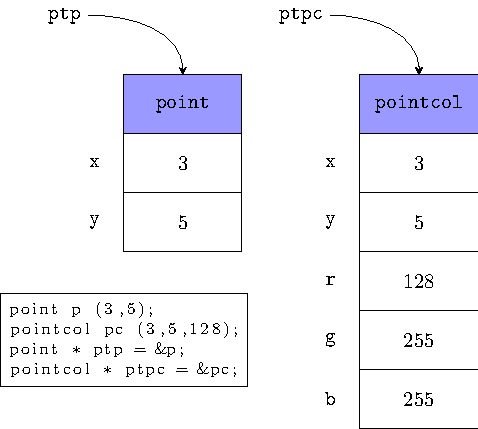
\includegraphics[height=5cm]{pics/link.pdf}}
%     \onslide<4>{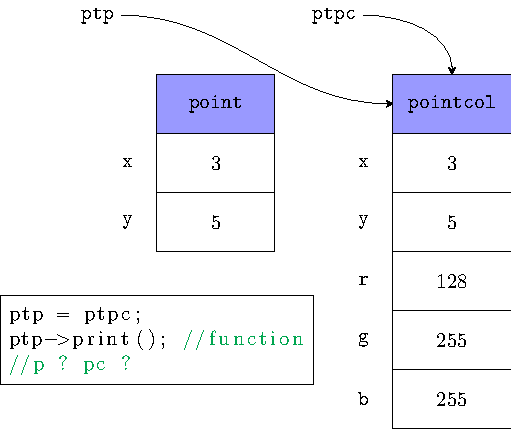
\includegraphics[height=5cm]{pics/link2.pdf}}
	\includegraphics<3|handout:0>[height=5cm]{pics/link.pdf}
	\includegraphics<4>[height=5cm]{pics/link2.pdf}
\end{overlayarea}
\end{center}
\end{frame}

\begin{frame}
\frametitle{Résolution statique des liens}
\begin{itemize}[<+->]
\item \texttt{ptp} est de type \texttt{point} mais l'objet pointé par \texttt{ptp} est de type \texttt{pointcol}.
	\begin{itemize}
	\item On choisit donc la fonction \texttt{print} de \texttt{point}
	\end{itemize}
\end{itemize}
\begin{exampleblock}<+->{Résolution statique des liens}
	\begin{itemize}[<+->]
	\item Le choix de la fonction est effectué à la compilation, une fois pour toutes
	\end{itemize}
\end{exampleblock}
\begin{itemize}[<+->]
\item Intuitivement, le type des objets pointés (ou non) est décidé et figé à la compilation.
\item Un choix de résolution ne peut-être effectué qu'avec des pointeurs et des références
	\begin{itemize}
	\item Avec des objets automatiques, un tronquage aurait été effectué
	\item Comportement indéterminé
	\end{itemize}
\end{itemize}
\end{frame}

\begin{frame}
\frametitle{Résolution dynamique des liens}
\begin{itemize}[<+->]
\item La fonction de la classe « la plus profonde » doit être appelée.
\end{itemize}
\begin{exampleblock}<+->{Résolution dynamique des liens}
	\begin{itemize}[<+->]
	\item La fonction à appeler doit être déterminée à l'exécution.
	\end{itemize}
\end{exampleblock}
\begin{itemize}[<+->]
\item Possible via des objets dynamiques et des méthodes virtuelles.
	\begin{itemize}
	\item Mot-clé \lstinline|virtual|
	\end{itemize}
\item Déclaration (suffisant) dans la classe de base.
\item Intuitivement : « tous les enfants définissent la fonction comme ils l'entendent ».
\end{itemize}
\end{frame}

\begin{frame}[containsverbatim]
\frametitle{Exemple}
\begin{itemize}
\item Fichier \texttt{dynamic.cpp}
\end{itemize}
\begin{lstlisting}
class point
{
	protected:
		int x, y;	
	public:
		point(int a = 0, int b = 0) : x(a), y(b) {}
		
		virtual void print()  {  cout << "( " << x << " , " << y << " )" << endl; }
};

class pointcol : public point
{
	short r, g, b;	
	
	public:
		pointcol(int x = 0, int y = 0, int r = 255, int g = 255, int b = 255) 
			: point(x,y), r(r), g(g), b(b) {}

		void print()
		{
			cout << "( " << x << " , " << y << " )" 
			     << " -- color " << r << " " << g << " " << b << endl;
		}
};
\end{lstlisting}
\end{frame}

\begin{frame}
\frametitle{Résolution dynamique des liens et polymorphisme}
\begin{itemize}[<+->]
\item Par défaut, toutes les résolutions de liens sont statiques.
	\begin{itemize}
	\item Performance
	\end{itemize}
\item \lstinline|virtual| impose une résolution dynamique des liens pour la fonction ainsi que toutes ses redéfinitions.	
	\begin{itemize}
	\item Légère perte de performance à l'exécution (runtime).
	\end{itemize}
\item On peut également faire de la détermination de type à l'exécution avec des objets dynamiques, sans tronquage.
\item Résolution dynamique des liens + résolution dynamique des types = polymorphisme.
\end{itemize}
\begin{alertblock}<+->{Remarque}
	\begin{itemize}
	\item Le polymorphisme ne s'applique jamais aux paramètres
	\end{itemize}
\end{alertblock}
\end{frame}

\begin{frame}[containsverbatim]
\frametitle{Exemple}
\begin{itemize}
\item Fichier \texttt{params.cpp}
\end{itemize}
\begin{lstlisting}
struct A
{
	virtual void f(A&) { cout << "A::f(A)" << endl; }
};

struct B : A
{
	virtual void f(A&) { cout << "B::f(A)" << endl; }
	virtual void f(B&) { cout << "B::f(B)" << endl; }
};

int main()
{
	A a; B b; A& ra = a;
	ra.f(a); ra.f(b);
	
	ra = b; ra.f(a); ra.f(b);
	
	A& rab = b; rab.f(a); rab.f(b);
	
	A * pa = new A; B * pb = new B;
	pa->f(*pa); pa->f(*pb);
	
	pa = pb; pa->f(*pa); pa->f(*pb);
}
\end{lstlisting}
\end{frame}

\begin{frame}
\frametitle{Debriefing}
\begin{itemize}[<+->]
\item \texttt{B::f(b)} n'est \emph{jamais} appelé
	\begin{itemize}
	\item Car c'est une surdéfinition, pas une redéfinition
%	\item Mot-clé \lstinline|override| (\cpp11)
	\end{itemize}
\end{itemize}
\begin{exampleblock}<+->{Rappel}
	\begin{itemize}[<+->]
	\item Les références sont \emph{constantes}
	\end{itemize}
\end{exampleblock}
\begin{itemize}[<+->]
\item Réaffecter une référence ne change pas la référence, mais l'objet référencé
\item Le type de l'objet référencé est déterminé dynamiquement (à l'exécution) lors de son initialisation
	\begin{itemize}
	\item Impossible de le changer après
	\end{itemize}
\item Ce genre de comportement « ne se produit pas » avec des pointeurs
	\begin{itemize}
	\item Émulation possible avec pointeurs constants
	\end{itemize}
\end{itemize}
\end{frame}

\begin{frame}
\frametitle{Le mot-clé \texttt{override}}
\begin{itemize}[<+->]
\item On peut préciser qu'une fonction dérivée redéfinit une fonction de base
\item Mot-clé \lstinline|override|
	\begin{itemize}
	\item Ex. : \lstinline|void f() override \{ ... \}|
	\end{itemize}
\item Facultatif, mais si on l'utilise pas, erreur de compilation
	\begin{itemize}
	\item Par ex., sur une surdéfinition
	\end{itemize}
\end{itemize}
\begin{exampleblock}<+->{Hygiène de programmation}
	\begin{itemize}[<+->]
	\item Utilisez le mot-clé \lstinline|override| à chaque fois que vous le pouvez
	\end{itemize}
\end{exampleblock}
\end{frame}

\begin{frame}
\frametitle{Opérateur d'affectation}
\begin{itemize}[<+->]
\item La surcharge d'opérateur peut être virtuelle.
\item L'affectation en particulier
	\begin{itemize}
	\item ... mais elle se comporte différemment d'une fonction « habituelle ».
	\end{itemize}
\item Redéfinir l'opérateur d'affectation dans une classe dérivée ne redéfinit pas l'opérateur d'affectation dans une classe de base.
	\begin{itemize}
	\item Parce que c'est une surdéfinition (paramètres différents)
	\end{itemize}
\end{itemize}
\begin{alertblock}<+->{Conclusion}
	\begin{itemize}[<+->]
	\item Le « polymorphisme » ne s'applique pas en cas d'affectation.
	\end{itemize}
\end{alertblock}
\end{frame}

\begin{frame}[containsverbatim]
\frametitle{Exemple}
\begin{itemize}
\item Fichier \texttt{affect-virtual.cpp}
\end{itemize}
\begin{lstlisting}
class A
{
	public:
		virtual A & operator = (const A&) { cout << "=A" << endl; }
};

class B : public A
{
	public:
		virtual B & operator = (const B&) //override //ko
		{ cout << "=B" << endl; }
};

int main()
{
	A * a1 = new A; A * a2 = new A;
	B * b1 = new B; B * b2 = new B;

	*b1 = *b2;
	*a1 = *b1;
	*a1 = *b2;
}
\end{lstlisting}
\begin{itemize}
\item Opérateur surdéfini, pas redéfini
\end{itemize}
\end{frame}

\begin{frame}
\frametitle{Propriétés des fonctions virtuelles}
\begin{itemize}[<+->]
\item Une fonction virtuelle dans une classe l'est dans toutes ses classes dérivées.
\item Redéfinir une fonction virtuelle n'est pas obligatoire.
\item On peut surdéfinir ($\neq$ redéfinir) une fonction virtuelle.
	\begin{itemize}
	\item ... mais c'est d'intérêt discutable.
	\end{itemize}
\item Le type de retour \texttt{R} ne peut pas être changé.
	\begin{itemize}
	\item ... sauf si on retourne un type dérivé de \texttt{R}
	\end{itemize}
\item Seule une fonction membre peut être virtuelle.
\item Un constructeur ne peut pas être virtuel.
	\begin{itemize}
	\item ... mais un destructeur, si.
	\end{itemize}
\item Attention : opérateur d'affectation.
	\begin{itemize}
	\item Pas de polymorphisme sur les paramètres
	\end{itemize}
\end{itemize}
\end{frame}

\begin{frame}
\frametitle{Destructeur virtuel}
\begin{block}<+->{Hygiène de programmation}
	\begin{itemize}[<+->]
	\item Dans une classe de base polymorphe, prévoir soit
		\begin{itemize}
		\item aucun destructeur,
		\item un destructeur privé ou protégé,
		\item un destructeur public virtuel.
		\end{itemize}
	\end{itemize}
\end{block}
\begin{exampleblock}<+->{Motivation}
	\begin{itemize}[<+->]
	\item Pour éviter une résolution statique des liens, soit on la « rend dynamique », soit on empêche la destruction.
	\end{itemize}
\end{exampleblock}
\begin{itemize}[<+->]
\item On veut absolument appeler les destructeurs des sous-classes 
	\begin{itemize}
	\item Idée : « éviter les ennuis »
	\end{itemize}
\end{itemize}
\end{frame}

\begin{frame}[containsverbatim]
\frametitle{Illustration}
\begin{itemize}
\item Fichier \texttt{destr-virt.cpp}
\end{itemize}
\begin{lstlisting}
struct Mere {
	~Mere() { cout << "-M" << endl; }
	virtual void print() { cout << "Mère " << endl; }	
};

struct Fille : Mere {
	~Fille() { cout << "-F" << endl; }
	void print() { cout << "Fille " << endl; }	
};

void print_indep(Mere* m) { m->print(); }

int main() {
	Mere * m = new Fille;
	print_indep(m);
    delete m;
}
\end{lstlisting}
\end{frame}

\begin{frame}
\frametitle{Fonctions virtuelles pures}
\begin{itemize}[<+->]
\item Idée : créer des classes \emph{abstraites} qui ne serviront qu'à être dérivées.
\item On peut forcer la redéfinition de certaines fonctions dont on ne connaît \emph{a priori} pas le comportement.
	\begin{itemize}
	\item Exemple : \texttt{sort} d'un algorithme de tri abstrait qui peut être implémenter par insertion, en bulle, etc.
	\end{itemize}
\item À l'évidence, ces classes ne peuvent être instanciées.
\item Utilisation de \emph{fonctions virtuelles pures}
	\begin{itemize}
	\item \lstinline|virtual void sort() = 0;|
	\end{itemize}
\item Définition \emph{nulle}, pas \emph{vide}.
\end{itemize}
\end{frame}

\begin{frame}
\frametitle{Classes abstraites}
\begin{itemize}[<+->]
\item Une classe comportant une fonction virtuelle pure est considérée comme \emph{abstraite}.
\item Une classe abstraite ne peut pas être instanciée
	\begin{itemize}
	\item ... mais on peut toujours avoir des objets dynamiques
	\item ... et des déclarations d'objets dynamiques.
	\end{itemize}
\item Motivation : polymorphisme
\item Une fonction virtuelle pure dans une classe de base doit obligatoirement être soit
	\begin{itemize}
	\item redéfinie dans les classes dérivées,
	\item déclarée à nouveau explicitement comme virtuelle pure dans les classes dérivées.
	\end{itemize}
\end{itemize}
\end{frame}

\begin{frame}[containsverbatim]
\frametitle{Exemple}
\begin{itemize}
\item Fichier \texttt{abstract.cpp}
\end{itemize}
\begin{lstlisting}
struct vehicle
{		
	virtual int nbWheels() = 0;
};

struct car : vehicle
{
	int nbWheels() override { return 4; }
};

struct bike : vehicle
{
	int nbWheels() override { return 2; }
};
\end{lstlisting}
\end{frame}

\begin{frame}[containsverbatim]
\frametitle{Exemple}
\begin{itemize}
\item Fichier \texttt{abstract.cpp}
\end{itemize}
\begin{lstlisting}
int main()
{
	car c;
	bike b;		

	cout << "Bike with " << b.nbWheels() << " wheels" << endl;
	cout << "Car with " << c.nbWheels() << " wheels" << endl;

	//vehicle v = bike(); //KO (instance)
	//vehicle v; //KO (instance)
	
	vehicle & rv = b; //ok
	cout << "Vehicle with " << rv.nbWheels() << " wheels" << endl;
	rv = c; //reaffacting a ref does not change the ref, but the referenced object
	cout << "Vehicle with " << rv.nbWheels() << " wheels" << endl;

	vehicle * v = new car();
	cout << "Vehicle with " << v -> nbWheels() << " wheels" << endl;
}
\end{lstlisting}
\end{frame}

\section{Héritage multiple}

\begin{frame}
\frametitle{Introduction}
\begin{itemize}[<+->]
\item Concrètement, permet à une classe d'être dérivée de plusieurs classes.
	\begin{itemize}
	\item Rappel : pas d'interfaces en \cpp.
	\end{itemize}
\item Les règles vues pour l'héritage « simple » sont d'application pour l'héritage multiple.
\item Mêmes « problèmes » liés à la résolution statique des liens, à la présence ou non de constructeurs de recopie, à la surcharge de l'affectation, etc.
\item Mêmes règles d'appel de constructeurs et de destructeurs.
	\begin{itemize}
	\item Quelques particularités toutefois.
	\end{itemize}
\item Mêmes manières d'appeler les fonctions et constructeurs des classes de base.
\end{itemize}
\end{frame}

\begin{frame}[containsverbatim]
\frametitle{Exemple}
\begin{itemize}
\item Fichier \texttt{multiple.cpp}
\end{itemize}
\begin{lstlisting}
class point
{
	int x, y;
	
	public:
		point(int a = 0, int b = 0) : x(a), y(b) {}

		virtual void print()
		{
			cout << "(" << x << " , " << y << ")";			
		}
};

class color
{
	short r, g, b;

	public:
		color(int r = 0, int g = 0, int b = 0) : r(r), g(g), b(b) {}

		virtual void print()
		{
			cout << "[" << r << " , " << g << " , " << b << "]";
		}
};
\end{lstlisting}
\end{frame}

\begin{frame}[containsverbatim]
\frametitle{Exemple}
\begin{itemize}
\item Fichier \texttt{multiple.cpp}
\end{itemize}
\begin{lstlisting}
class pointcol : public point, public color
{	
	public:
		pointcol(int x = 0, int y = 0, int r = 0, int g = 0, int b = 0) 
			: point(x,y), color(r,g,b) {}

		void print() override
		{
			cout << "{ "; 
			point::print(); cout << " , "; color::print();
			cout << " }";
		}
};

int main()
{
	pointcol p(1,2,100,128,255);
	p.print(); cout << endl;
	p.point::print(); cout << endl;
	p.color::print(); cout << endl;
	
	color & c = p; c.print(); cout << endl;	
	point& pp = p; pp.print(); cout << endl;
}
\end{lstlisting}
\end{frame}


\begin{frame}
\frametitle{Appel des constructeurs et destructeurs}
\begin{exampleblock}<+->{Héritage simple}
	\begin{itemize}[<+->]
	\item Constructeurs : ordre de dérivation (base > dérivée).
	\item Destructeurs : ordre inverse de dérivation (dérivée > base).
	\end{itemize}
\end{exampleblock}
\begin{exampleblock}<+->{Héritage multiple}
	\begin{itemize}[<+->]
	\item Constructeurs : ordre de dérivation, par ordre de déclaration (base1 > base2 > dérivée).
	\item Destructeurs : ordre inverse de dérivation, par ordre inverse de déclaration (dérivée > base2 > base1).
	\end{itemize}
\end{exampleblock}
\end{frame}

\begin{frame}[containsverbatim]
\begin{itemize}
\item Fichier \texttt{cstr-mult.cpp}
\end{itemize}
\begin{lstlisting}
struct A
{
	A() { cout << "+A" << endl; }
	A(const A& a) { cout << "rA" << endl; }
	virtual ~A() { cout << "-A" << endl; }
};

struct B
{
	B() { cout << "+B" << endl; }
	B(const B& a) { cout << "rB" << endl; }
	virtual ~B() { cout << "-B" << endl; }
};

struct C : A, B
{
	C() { cout << "+C" << endl; }
	C(const C& a) { cout << "rC" << endl; }
	virtual ~C() { cout << "-C" << endl; }
};

void f(A a) {}

int main()
{
	C c; cout << endl;
	f(c); cout << endl;
	C * cc = new C(); cout << endl;
	delete cc; cout << endl;
}
\end{lstlisting}
\end{frame}

\begin{frame}
\frametitle{Problème lié à l'héritage multiple}
\begin{itemize}
\onslide<1-> \item Supposez qu'on ait le schéma de dérivation suivant
\end{itemize}
\begin{center}
\visible<2-|handout:1>{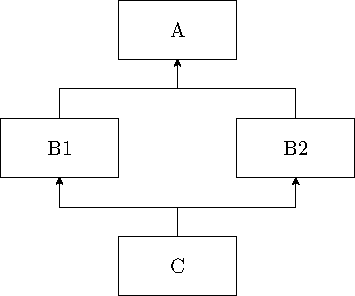
\includegraphics[width=3.5cm]{pics/diamond.pdf}}
\end{center}
\onslide<3-> 
\begin{exampleblock}{Question}
	\begin{itemize}
	\onslide<4-> \item Que fait un appel depuis \texttt{C} à un attribut de \texttt{A}, si \texttt{B1} et \texttt{B2} ne construisent pas \texttt{A} de la même façon ?
	\end{itemize}
\end{exampleblock}
\end{frame}

\begin{frame}[containsverbatim]
\begin{itemize}
\item Fichier \texttt{diamond.cpp}
\end{itemize}
\begin{lstlisting}
struct A
{
	int i;
	A(int i = 0) : i(i) {}
};

struct B1 : A
{
	B1(int j = 0) : A(j) {}
};

struct B2 : A
{
	B2(int j = 0) : A(j) {}
};

struct C : B1, B2
{
	C(int j1 = 0, int j2 = 0) : B1(j1), B2(j2) {}
};

int main()
{
	C c (2, 4);
	cout << c.i << endl; //?!
}
\end{lstlisting}
\end{frame}

\begin{frame}
\frametitle{Diamond of DEATH : le problème}
\begin{itemize}
\onslide<1-> \item On remarque que la classe \texttt{C} possède deux copies de «~super-objets~» de types \texttt{A}
\onslide<2-> \item Ces super-objets sont distincts, avec des attributs distincts
\end{itemize}
\begin{center}
\visible<3-|handout:1>{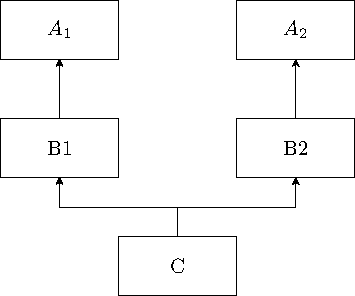
\includegraphics[width=4cm]{pics/diamond2.pdf}}
\end{center}
\begin{itemize}
\onslide<4-> \item L'appel \texttt{c.i} est ambigu.
	\begin{itemize}
	\onslide<5-> \item On ne sait pas quel « chemin de dérivation » privilégier.
	\end{itemize}
\onslide<6-> \item Ordre d'appel des constructeurs : $A_1~B1~A_2~B2~C$
\end{itemize}
\end{frame}

\begin{frame}
\frametitle{Dérivation « virtuelle »}
\begin{itemize}[<+->]
\item L'héritage multiple peut conduire à une duplication des membres.
	\begin{itemize}
	\item Attributs : problématique.
	\item Fonctions : moins d'importance (résolution de portée).
	\end{itemize}
\item En général, on ne veut délibérément une duplication des attributs
	\begin{itemize}
	\item Bonne pratique ? Synchronisation ?
	\end{itemize}
\item On pourrait ne travailler qu'avec un jeu de données
	\begin{itemize}
	\item Pertinence ? Synchronisation ?
	\end{itemize}
\end{itemize}
\begin{exampleblock}<+->{Solution : « dérivation virtuelle »}
	\begin{itemize}
	\item \lstinline|class B1 : public virtual A|
	\item \lstinline|class B2 : public virtual A|
	\item \lstinline|class C : public B1, public B2|
	\end{itemize}
\end{exampleblock}
\end{frame}

\begin{frame}
\frametitle{Construction : transmission des arguments}
\begin{alertblock}<+->{Problème}
\begin{itemize}[<+->]
\item Quels arguments transmettre au constructeur ? Ceux de \texttt{B1} ou ceux de \texttt{B2} ?
\end{itemize}
\end{alertblock}
\begin{exampleblock}<+->{Solution}
\begin{itemize}[<+->]
\item En cas de dérivation virtuelle \emph{uniquement}, on peut spécifier dans \texttt{C} des informations destinées à \texttt{A}.
\end{itemize}
\end{exampleblock}
\begin{itemize}[<+->]
\item Exemple : \lstinline|C(int j1, int j2) : A((j1 + j2) / 2, ... \{\}|
\end{itemize}
\end{frame}

\begin{frame}[containsverbatim]
\begin{itemize}
\item Fichier \texttt{diamond2.cpp}
\end{itemize}
\begin{lstlisting}
struct A
{
	int i;
	A(int i = 0) : i(i) {}
};

struct B1 : virtual A
{
	B1(int j = 0) : A(j) {}
};

struct B2 : virtual A
{
	B2(int j = 0) : A(j) {}
};

struct C : B1, B2
{
	C(int j1 = 0, int j2 = 0) : A((j1 + j2) / 2, B1(j1), B2(j2) {}
};

int main()
{
	C c (2, 4);
	cout << c.i << endl;
	cout << c.B1::i << endl;
	cout << c.B2::i << endl;
}
\end{lstlisting}
\end{frame}

\begin{frame}
\frametitle{Remarque}
\begin{itemize}[<+->]
	\item Ordre d'appel : le constructeur d'une classe virtuelle est toujours appelé avant les autres.
	\item Exemple précédent : $A~B1~B2~C$.
\end{itemize}
\begin{block}<+->{Hygiène de programmation}
\begin{itemize}[<+->]
\item Hériter «~comme en Java~»
	\begin{itemize}
	\item Ne pas avoir de «~diamant~»,
	\item Ne pas hériter multiplement s'il y a des attributs en commun
	\end{itemize}
\end{itemize}
\end{block}
\begin{itemize}[<+->]
\item Motivation : pouvoir instancier « correctement et pertinemment » les classes de type \texttt{B1} ou \texttt{B2}.
%	\begin{itemize}
%	\item «~Incohérence~» : fichier \texttt{diamond-3.cpp}
%	\end{itemize}
\end{itemize}
\end{frame}
\end{document}
